\documentclass[1p]{elsarticle_modified}
%\bibliographystyle{elsarticle-num}

%\usepackage[colorlinks]{hyperref}
%\usepackage{abbrmath_seonhwa} %\Abb, \Ascr, \Acal ,\Abf, \Afrak
\usepackage{amsfonts}
\usepackage{amssymb}
\usepackage{amsmath}
\usepackage{amsthm}
\usepackage{scalefnt}
\usepackage{amsbsy}
\usepackage{kotex}
\usepackage{caption}
\usepackage{subfig}
\usepackage{color}
\usepackage{graphicx}
\usepackage{xcolor} %% white, black, red, green, blue, cyan, magenta, yellow
\usepackage{float}
\usepackage{setspace}
\usepackage{hyperref}

\usepackage{tikz}
\usetikzlibrary{arrows}

\usepackage{multirow}
\usepackage{array} % fixed length table
\usepackage{hhline}

%%%%%%%%%%%%%%%%%%%%%
\makeatletter
\renewcommand*\env@matrix[1][\arraystretch]{%
	\edef\arraystretch{#1}%
	\hskip -\arraycolsep
	\let\@ifnextchar\new@ifnextchar
	\array{*\c@MaxMatrixCols c}}
\makeatother %https://tex.stackexchange.com/questions/14071/how-can-i-increase-the-line-spacing-in-a-matrix
%%%%%%%%%%%%%%%

\usepackage[normalem]{ulem}

\newcommand{\msout}[1]{\ifmmode\text{\sout{\ensuremath{#1}}}\else\sout{#1}\fi}
%SOURCE: \msout is \stkout macro in https://tex.stackexchange.com/questions/20609/strikeout-in-math-mode

\newcommand{\cancel}[1]{
	\ifmmode
	{\color{red}\msout{#1}}
	\else
	{\color{red}\sout{#1}}
	\fi
}

\newcommand{\add}[1]{
	{\color{blue}\uwave{#1}}
}

\newcommand{\replace}[2]{
	\ifmmode
	{\color{red}\msout{#1}}{\color{blue}\uwave{#2}}
	\else
	{\color{red}\sout{#1}}{\color{blue}\uwave{#2}}
	\fi
}

\newcommand{\Sol}{\mathcal{S}} %segment
\newcommand{\D}{D} %diagram
\newcommand{\A}{\mathcal{A}} %arc


%%%%%%%%%%%%%%%%%%%%%%%%%%%%%5 test

\def\sl{\operatorname{\textup{SL}}(2,\Cbb)}
\def\psl{\operatorname{\textup{PSL}}(2,\Cbb)}
\def\quan{\mkern 1mu \triangleright \mkern 1mu}

\theoremstyle{definition}
\newtheorem{thm}{Theorem}[section]
\newtheorem{prop}[thm]{Proposition}
\newtheorem{lem}[thm]{Lemma}
\newtheorem{ques}[thm]{Question}
\newtheorem{cor}[thm]{Corollary}
\newtheorem{defn}[thm]{Definition}
\newtheorem{exam}[thm]{Example}
\newtheorem{rmk}[thm]{Remark}
\newtheorem{alg}[thm]{Algorithm}

\newcommand{\I}{\sqrt{-1}}
\begin{document}

%\begin{frontmatter}
%
%\title{Boundary parabolic representations of knots up to 8 crossings}
%
%%% Group authors per affiliation:
%\author{Yunhi Cho} 
%\address{Department of Mathematics, University of Seoul, Seoul, Korea}
%\ead{yhcho@uos.ac.kr}
%
%
%\author{Seonhwa Kim} %\fnref{s_kim}}
%\address{Center for Geometry and Physics, Institute for Basic Science, Pohang, 37673, Korea}
%\ead{ryeona17@ibs.re.kr}
%
%\author{Hyuk Kim}
%\address{Department of Mathematical Sciences, Seoul National University, Seoul 08826, Korea}
%\ead{hyukkim@snu.ac.kr}
%
%\author{Seokbeom Yoon}
%\address{Department of Mathematical Sciences, Seoul National University, Seoul, 08826,  Korea}
%\ead{sbyoon15@snu.ac.kr}
%
%\begin{abstract}
%We find all boundary parabolic representation of knots up to 8 crossings.
%
%\end{abstract}
%\begin{keyword}
%    \MSC[2010] 57M25 
%\end{keyword}
%
%\end{frontmatter}

%\linenumbers
%\tableofcontents
%
\newcommand\colored[1]{\textcolor{white}{\rule[-0.35ex]{0.8em}{1.4ex}}\kern-0.8em\color{red} #1}%
%\newcommand\colored[1]{\textcolor{white}{ #1}\kern-2.17ex	\textcolor{white}{ #1}\kern-1.81ex	\textcolor{white}{ #1}\kern-2.15ex\color{red}#1	}

{\Large $\underline{11n_{127}~(K11n_{127})}$}

\setlength{\tabcolsep}{10pt}
\renewcommand{\arraystretch}{1.6}
\vspace{1cm}\begin{tabular}{m{100pt}>{\centering\arraybackslash}m{274pt}}
\multirow{5}{120pt}{
	\centering
	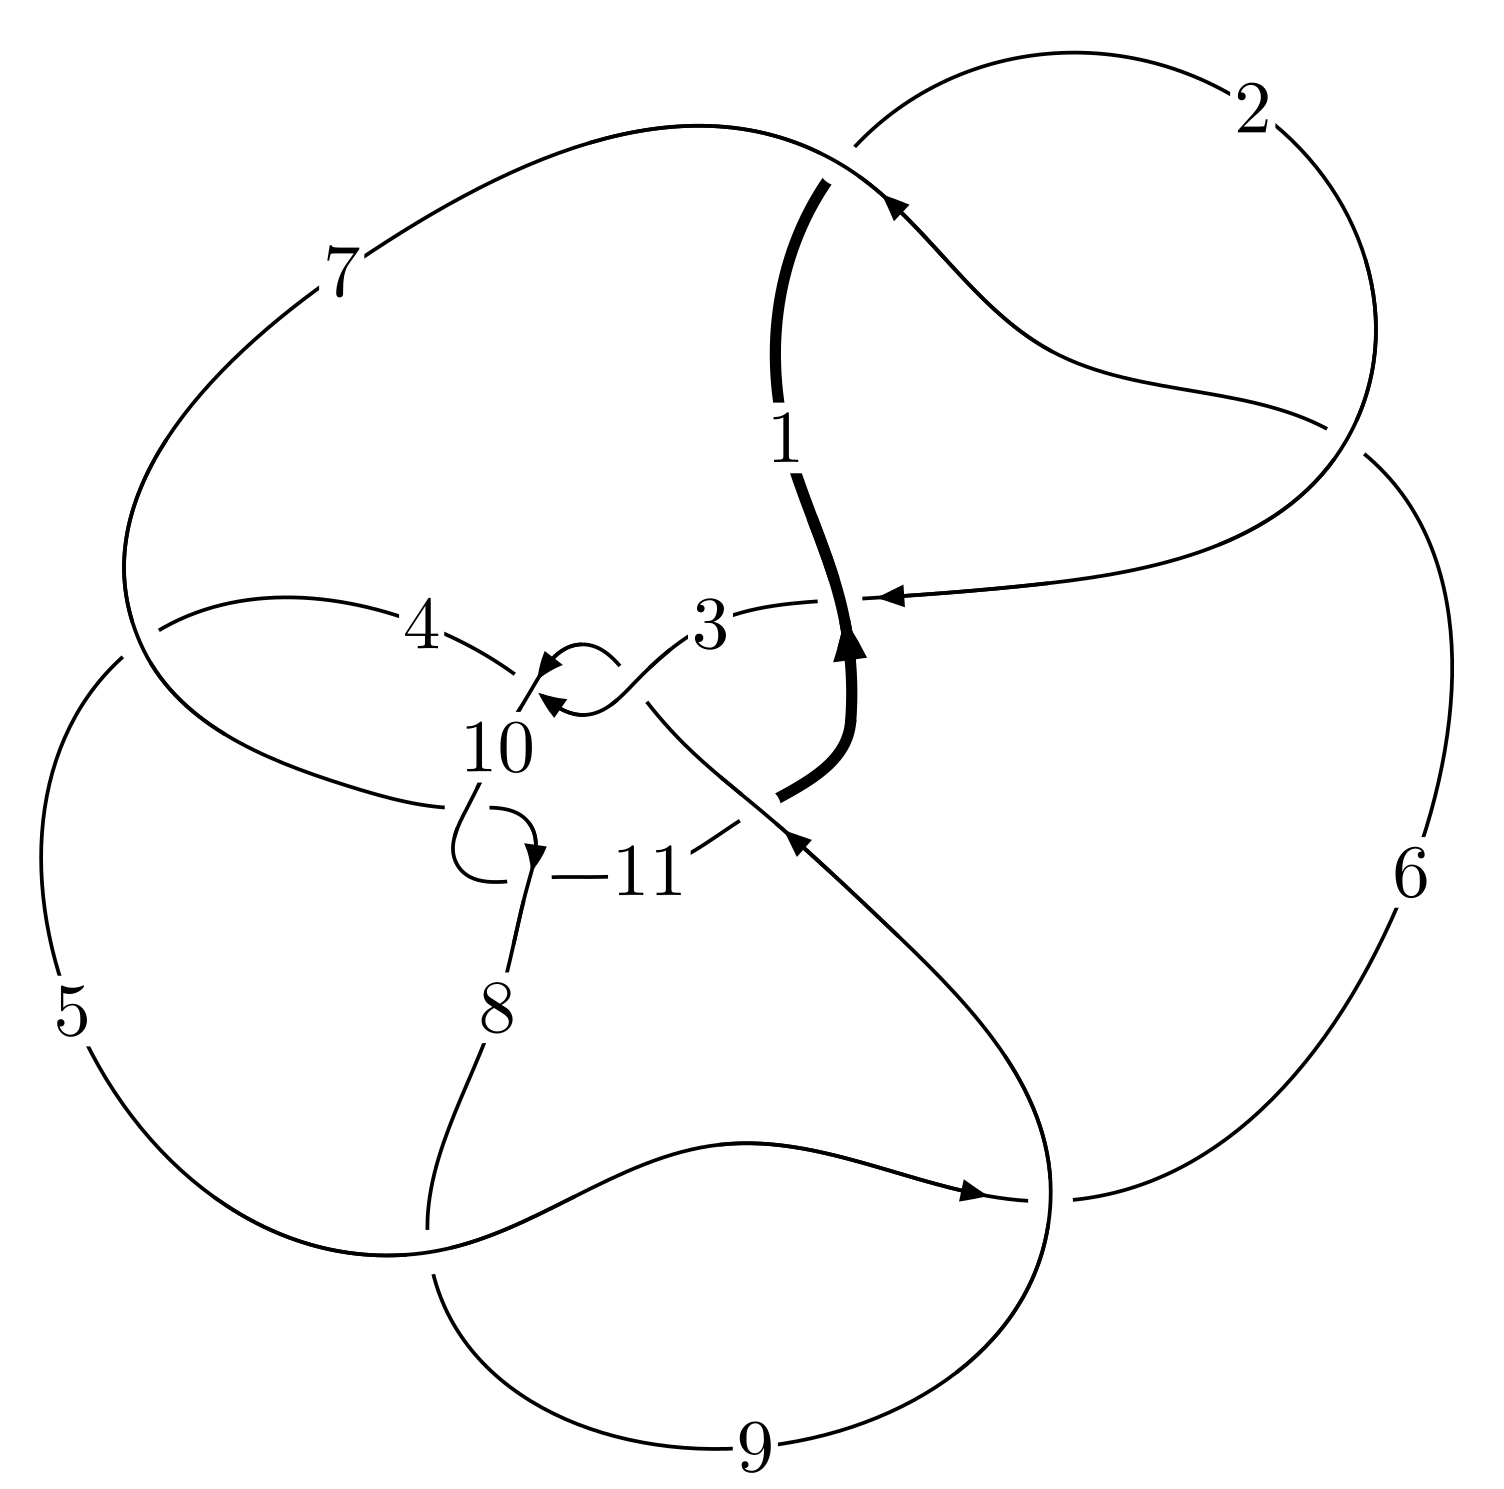
\includegraphics[width=112pt]{../../../GIT/diagram.site/Diagrams/png/743_11n_127.png}\\
\ \ \ A knot diagram\footnotemark}&
\allowdisplaybreaks
\textbf{Linearized knot diagam} \\
\cline{2-2}
 &
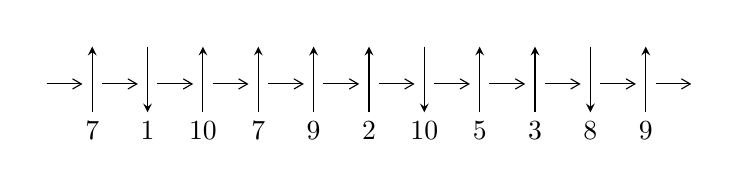
\begin{tikzpicture}[x=20pt, y=17pt]
	% nodes
	\node (C0) at (0, 0) {};
	\node (C1) at (1, 0) {};
	\node (C1U) at (1, +1) {};
	\node (C1D) at (1, -1) {7};

	\node (C2) at (2, 0) {};
	\node (C2U) at (2, +1) {};
	\node (C2D) at (2, -1) {1};

	\node (C3) at (3, 0) {};
	\node (C3U) at (3, +1) {};
	\node (C3D) at (3, -1) {10};

	\node (C4) at (4, 0) {};
	\node (C4U) at (4, +1) {};
	\node (C4D) at (4, -1) {7};

	\node (C5) at (5, 0) {};
	\node (C5U) at (5, +1) {};
	\node (C5D) at (5, -1) {9};

	\node (C6) at (6, 0) {};
	\node (C6U) at (6, +1) {};
	\node (C6D) at (6, -1) {2};

	\node (C7) at (7, 0) {};
	\node (C7U) at (7, +1) {};
	\node (C7D) at (7, -1) {10};

	\node (C8) at (8, 0) {};
	\node (C8U) at (8, +1) {};
	\node (C8D) at (8, -1) {5};

	\node (C9) at (9, 0) {};
	\node (C9U) at (9, +1) {};
	\node (C9D) at (9, -1) {3};

	\node (C10) at (10, 0) {};
	\node (C10U) at (10, +1) {};
	\node (C10D) at (10, -1) {8};

	\node (C11) at (11, 0) {};
	\node (C11U) at (11, +1) {};
	\node (C11D) at (11, -1) {9};
	\node (C12) at (12, 0) {};

	% arrows
	\draw[->,>={angle 60}]
	(C0) edge (C1) (C1) edge (C2) (C2) edge (C3) (C3) edge (C4) (C4) edge (C5) (C5) edge (C6) (C6) edge (C7) (C7) edge (C8) (C8) edge (C9) (C9) edge (C10) (C10) edge (C11) (C11) edge (C12) ;	\draw[->,>=stealth]
	(C1D) edge (C1U) (C2U) edge (C2D) (C3D) edge (C3U) (C4D) edge (C4U) (C5D) edge (C5U) (C6D) edge (C6U) (C7U) edge (C7D) (C8D) edge (C8U) (C9D) edge (C9U) (C10U) edge (C10D) (C11D) edge (C11U) ;
	\end{tikzpicture} \\
\hhline{~~} \\& 
\textbf{Solving Sequence} \\ \cline{2-2} 
 &
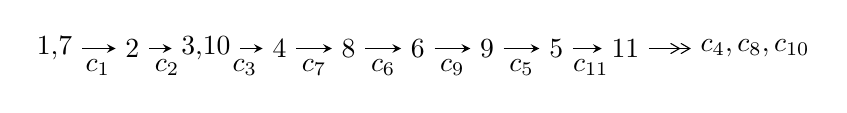
\begin{tikzpicture}[x=25pt, y=7pt]
	% node
	\node (A0) at (-1/8, 0) {1,7};
	\node (A1) at (1, 0) {2};
	\node (A2) at (33/16, 0) {3,10};
	\node (A3) at (25/8, 0) {4};
	\node (A4) at (33/8, 0) {8};
	\node (A5) at (41/8, 0) {6};
	\node (A6) at (49/8, 0) {9};
	\node (A7) at (57/8, 0) {5};
	\node (A8) at (65/8, 0) {11};
	\node (C1) at (1/2, -1) {$c_{1}$};
	\node (C2) at (3/2, -1) {$c_{2}$};
	\node (C3) at (21/8, -1) {$c_{3}$};
	\node (C4) at (29/8, -1) {$c_{7}$};
	\node (C5) at (37/8, -1) {$c_{6}$};
	\node (C6) at (45/8, -1) {$c_{9}$};
	\node (C7) at (53/8, -1) {$c_{5}$};
	\node (C8) at (61/8, -1) {$c_{11}$};
	\node (A9) at (10, 0) {$c_{4},c_{8},c_{10}$};

	% edge
	\draw[->,>=stealth]	
	(A0) edge (A1) (A1) edge (A2) (A2) edge (A3) (A3) edge (A4) (A4) edge (A5) (A5) edge (A6) (A6) edge (A7) (A7) edge (A8) ;
	\draw[->>,>={angle 60}]	
	(A8) edge (A9);
\end{tikzpicture} \\ 

\end{tabular} \\

\footnotetext{
The image of knot diagram is generated by the software ``\textbf{Draw programme}" developed by Andrew Bartholomew(\url{http://www.layer8.co.uk/maths/draw/index.htm\#Running-draw}), where we modified some parts for our purpose(\url{https://github.com/CATsTAILs/LinksPainter}).
}\phantom \\ \newline 
\centering \textbf{Ideals for irreducible components\footnotemark of $X_{\text{par}}$} 
 
\begin{align*}
I^u_{1}&=\langle 
- u^{15}+6 u^{14}+\cdots+2 b-11 u,\;- u^{15}+3 u^{14}+\cdots+2 a+11,\;u^{16}-4 u^{15}+\cdots-14 u+4\rangle \\
I^u_{2}&=\langle 
u^8+2 u^7+4 u^6+5 u^5+6 u^4+6 u^3+3 u^2+b+2 u+1,\;u^7+u^6+2 u^5+u^4+2 u^3+2 u^2+a,\\
\phantom{I^u_{2}}&\phantom{= \langle  }u^9+u^8+3 u^7+2 u^6+4 u^5+3 u^4+2 u^3+2 u^2+1\rangle \\
I^u_{3}&=\langle 
2 u^3 b a-2 u^4 a+u^2 b a-2 u^3 a+2 b a u-2 u^2 a+b^2+2 b a- a u+u^2+2 u+1,\\
\phantom{I^u_{3}}&\phantom{= \langle  }u^4 a+u^3 a- u^4+2 u^2 a+a^2+a u- u^2+a+u,\;u^5+u^4+2 u^3+u^2+u+1\rangle \\
\\
\end{align*}
\raggedright * 3 irreducible components of $\dim_{\mathbb{C}}=0$, with total 45 representations.\\
\footnotetext{All coefficients of polynomials are rational numbers. But the coefficients are sometimes approximated in decimal forms when there is not enough margin.}
\newpage
\renewcommand{\arraystretch}{1}
\centering \section*{I. $I^u_{1}= \langle - u^{15}+6 u^{14}+\cdots+2 b-11 u,\;- u^{15}+3 u^{14}+\cdots+2 a+11,\;u^{16}-4 u^{15}+\cdots-14 u+4 \rangle$}
\flushleft \textbf{(i) Arc colorings}\\
\begin{tabular}{m{7pt} m{180pt} m{7pt} m{180pt} }
\flushright $a_{1}=$&$\begin{pmatrix}1\\0\end{pmatrix}$ \\
\flushright $a_{7}=$&$\begin{pmatrix}0\\u\end{pmatrix}$ \\
\flushright $a_{2}=$&$\begin{pmatrix}1\\- u^2\end{pmatrix}$ \\
\flushright $a_{3}=$&$\begin{pmatrix}u^2+1\\- u^2\end{pmatrix}$ \\
\flushright $a_{10}=$&$\begin{pmatrix}\frac{1}{2} u^{15}-\frac{3}{2} u^{14}+\cdots+13 u-\frac{11}{2}\\\frac{1}{2} u^{15}-3 u^{14}+\cdots-\frac{23}{2} u^2+\frac{11}{2} u\end{pmatrix}$ \\
\flushright $a_{4}=$&$\begin{pmatrix}\frac{3}{4} u^{15}-\frac{5}{2} u^{14}+\cdots+\frac{27}{4} u-2\\-\frac{1}{2} u^{15}+2 u^{14}+\cdots-\frac{7}{2} u+1\end{pmatrix}$ \\
\flushright $a_{8}=$&$\begin{pmatrix}\frac{1}{4} u^{15}+\frac{1}{2} u^{14}+\cdots-\frac{27}{4} u+3\\-\frac{1}{2} u^{15}+u^{14}+\cdots+\frac{1}{2} u-1\end{pmatrix}$ \\
\flushright $a_{6}=$&$\begin{pmatrix}- u\\u^3+u\end{pmatrix}$ \\
\flushright $a_{9}=$&$\begin{pmatrix}-\frac{3}{2} u^{14}+5 u^{13}+\cdots+\frac{33}{2} u-\frac{15}{2}\\\frac{3}{2} u^{15}-5 u^{14}+\cdots-\frac{33}{2} u^2+\frac{15}{2} u\end{pmatrix}$ \\
\flushright $a_{5}=$&$\begin{pmatrix}\frac{3}{4} u^{15}-\frac{5}{2} u^{14}+\cdots+\frac{27}{4} u-2\\-\frac{1}{2} u^{15}+2 u^{14}+\cdots-\frac{15}{2} u+3\end{pmatrix}$ \\
\flushright $a_{11}=$&$\begin{pmatrix}\frac{1}{4} u^{15}+\frac{1}{2} u^{14}+\cdots-\frac{23}{4} u+4\\-\frac{3}{2} u^{15}+4 u^{14}+\cdots-\frac{13}{2} u+1\end{pmatrix}$\\ \flushright $a_{11}=$&$\begin{pmatrix}\frac{1}{4} u^{15}+\frac{1}{2} u^{14}+\cdots-\frac{23}{4} u+4\\-\frac{3}{2} u^{15}+4 u^{14}+\cdots-\frac{13}{2} u+1\end{pmatrix}$\\&\end{tabular}
\flushleft \textbf{(ii) Obstruction class $= -1$}\\~\\
\flushleft \textbf{(iii) Cusp Shapes $= u^{15}+2 u^{14}-4 u^{13}+18 u^{12}-23 u^{11}+36 u^{10}-42 u^9+49 u^8-57 u^7+38 u^6-17 u^5+6 u^4-4 u^3+23 u^2-14 u+6$}\\~\\
\newpage\renewcommand{\arraystretch}{1}
\flushleft \textbf{(iv) u-Polynomials at the component}\newline \\
\begin{tabular}{m{50pt}|m{274pt}}
Crossings & \hspace{64pt}u-Polynomials at each crossing \\
\hline $$\begin{aligned}c_{1},c_{6}\end{aligned}$$&$\begin{aligned}
&u^{16}+4 u^{15}+\cdots+14 u+4
\end{aligned}$\\
\hline $$\begin{aligned}c_{2}\end{aligned}$$&$\begin{aligned}
&u^{16}+8 u^{15}+\cdots-12 u+16
\end{aligned}$\\
\hline $$\begin{aligned}c_{3},c_{5},c_{8}\\c_{9}\end{aligned}$$&$\begin{aligned}
&u^{16}- u^{15}+\cdots- u+1
\end{aligned}$\\
\hline $$\begin{aligned}c_{4}\end{aligned}$$&$\begin{aligned}
&u^{16}+u^{15}+\cdots- u+1
\end{aligned}$\\
\hline $$\begin{aligned}c_{7},c_{10}\end{aligned}$$&$\begin{aligned}
&u^{16}-9 u^{15}+\cdots-128 u+32
\end{aligned}$\\
\hline $$\begin{aligned}c_{11}\end{aligned}$$&$\begin{aligned}
&u^{16}+3 u^{15}+\cdots- u+1
\end{aligned}$\\
\hline
\end{tabular}\\~\\
\newpage\renewcommand{\arraystretch}{1}
\flushleft \textbf{(v) Riley Polynomials at the component}\newline \\
\begin{tabular}{m{50pt}|m{274pt}}
Crossings & \hspace{64pt}Riley Polynomials at each crossing \\
\hline $$\begin{aligned}c_{1},c_{6}\end{aligned}$$&$\begin{aligned}
&y^{16}+8 y^{15}+\cdots-12 y+16
\end{aligned}$\\
\hline $$\begin{aligned}c_{2}\end{aligned}$$&$\begin{aligned}
&y^{16}+20 y^{14}+\cdots+784 y+256
\end{aligned}$\\
\hline $$\begin{aligned}c_{3},c_{5},c_{8}\\c_{9}\end{aligned}$$&$\begin{aligned}
&y^{16}+y^{15}+\cdots-5 y+1
\end{aligned}$\\
\hline $$\begin{aligned}c_{4}\end{aligned}$$&$\begin{aligned}
&y^{16}+29 y^{15}+\cdots+31 y+1
\end{aligned}$\\
\hline $$\begin{aligned}c_{7},c_{10}\end{aligned}$$&$\begin{aligned}
&y^{16}-13 y^{15}+\cdots-512 y+1024
\end{aligned}$\\
\hline $$\begin{aligned}c_{11}\end{aligned}$$&$\begin{aligned}
&y^{16}+17 y^{15}+\cdots-21 y+1
\end{aligned}$\\
\hline
\end{tabular}\\~\\
\newpage\flushleft \textbf{(vi) Complex Volumes and Cusp Shapes}
$$\begin{array}{c|c|c}  
\text{Solutions to }I^u_{1}& \I (\text{vol} + \sqrt{-1}CS) & \text{Cusp shape}\\
 \hline 
\begin{aligned}
u &= \phantom{-}0.942369 + 0.202951 I \\
a &= -1.72389 - 0.04762 I \\
b &= \phantom{-}0.379524 + 0.857765 I\end{aligned}
 & -6.09218 - 7.65352 I & \phantom{-}5.03016 + 4.26371 I \\ \hline\begin{aligned}
u &= \phantom{-}0.942369 - 0.202951 I \\
a &= -1.72389 + 0.04762 I \\
b &= \phantom{-}0.379524 - 0.857765 I\end{aligned}
 & -6.09218 + 7.65352 I & \phantom{-}5.03016 - 4.26371 I \\ \hline\begin{aligned}
u &= \phantom{-}0.278245 + 1.091110 I \\
a &= \phantom{-}0.701786 - 0.590992 I \\
b &= -0.528417 - 0.110176 I\end{aligned}
 & -3.59071 + 0.23489 I & \phantom{-}0.00495 + 2.03163 I \\ \hline\begin{aligned}
u &= \phantom{-}0.278245 - 1.091110 I \\
a &= \phantom{-}0.701786 + 0.590992 I \\
b &= -0.528417 + 0.110176 I\end{aligned}
 & -3.59071 - 0.23489 I & \phantom{-}0.00495 - 2.03163 I \\ \hline\begin{aligned}
u &= -0.666650 + 0.457955 I \\
a &= \phantom{-}0.813008 - 0.264852 I \\
b &= \phantom{-}0.209000 + 0.442237 I\end{aligned}
 & \phantom{-}1.227240 - 0.533814 I & \phantom{-}8.87917 + 3.72662 I \\ \hline\begin{aligned}
u &= -0.666650 - 0.457955 I \\
a &= \phantom{-}0.813008 + 0.264852 I \\
b &= \phantom{-}0.209000 - 0.442237 I\end{aligned}
 & \phantom{-}1.227240 + 0.533814 I & \phantom{-}8.87917 - 3.72662 I \\ \hline\begin{aligned}
u &= \phantom{-}0.709198 + 0.345008 I \\
a &= \phantom{-}0.992942 + 0.950055 I \\
b &= \phantom{-}0.076805 - 1.100350 I\end{aligned}
 & \phantom{-}0.53868 - 2.34706 I & \phantom{-}5.73269 + 5.07520 I \\ \hline\begin{aligned}
u &= \phantom{-}0.709198 - 0.345008 I \\
a &= \phantom{-}0.992942 - 0.950055 I \\
b &= \phantom{-}0.076805 + 1.100350 I\end{aligned}
 & \phantom{-}0.53868 + 2.34706 I & \phantom{-}5.73269 - 5.07520 I \\ \hline\begin{aligned}
u &= \phantom{-}0.555419 + 1.111790 I \\
a &= -0.674901 - 0.885563 I \\
b &= -0.72750 + 1.84198 I\end{aligned}
 & -1.69676 + 7.19836 I & \phantom{-}2.21492 - 9.55770 I \\ \hline\begin{aligned}
u &= \phantom{-}0.555419 - 1.111790 I \\
a &= -0.674901 + 0.885563 I \\
b &= -0.72750 - 1.84198 I\end{aligned}
 & -1.69676 - 7.19836 I & \phantom{-}2.21492 + 9.55770 I\\
 \hline 
 \end{array}$$\newpage$$\begin{array}{c|c|c}  
\text{Solutions to }I^u_{1}& \I (\text{vol} + \sqrt{-1}CS) & \text{Cusp shape}\\
 \hline 
\begin{aligned}
u &= -0.706391 + 1.042180 I \\
a &= \phantom{-}0.131675 + 0.901270 I \\
b &= -0.95468 - 1.04353 I\end{aligned}
 & -0.51238 - 4.79975 I & \phantom{-}9.59566 + 5.34793 I \\ \hline\begin{aligned}
u &= -0.706391 - 1.042180 I \\
a &= \phantom{-}0.131675 - 0.901270 I \\
b &= -0.95468 + 1.04353 I\end{aligned}
 & -0.51238 + 4.79975 I & \phantom{-}9.59566 - 5.34793 I \\ \hline\begin{aligned}
u &= \phantom{-}0.572643 + 1.229640 I \\
a &= -0.261905 + 1.244920 I \\
b &= \phantom{-}1.82806 - 2.11251 I\end{aligned}
 & -9.2176 + 13.1290 I & \phantom{-}2.40989 - 7.11896 I \\ \hline\begin{aligned}
u &= \phantom{-}0.572643 - 1.229640 I \\
a &= -0.261905 - 1.244920 I \\
b &= \phantom{-}1.82806 + 2.11251 I\end{aligned}
 & -9.2176 - 13.1290 I & \phantom{-}2.40989 + 7.11896 I \\ \hline\begin{aligned}
u &= \phantom{-}0.315167 + 1.323970 I \\
a &= -0.478712 + 1.077590 I \\
b &= \phantom{-}0.217216 - 1.305260 I\end{aligned}
 & -11.08760 - 3.34610 I & \phantom{-}0.13256 + 2.28731 I \\ \hline\begin{aligned}
u &= \phantom{-}0.315167 - 1.323970 I \\
a &= -0.478712 - 1.077590 I \\
b &= \phantom{-}0.217216 + 1.305260 I\end{aligned}
 & -11.08760 + 3.34610 I & \phantom{-}0.13256 - 2.28731 I\\
 \hline 
 \end{array}$$\newpage\newpage\renewcommand{\arraystretch}{1}
\centering \section*{II. $I^u_{2}= \langle u^8+2 u^7+\cdots+b+1,\;u^7+u^6+2 u^5+u^4+2 u^3+2 u^2+a,\;u^9+u^8+\cdots+2 u^2+1 \rangle$}
\flushleft \textbf{(i) Arc colorings}\\
\begin{tabular}{m{7pt} m{180pt} m{7pt} m{180pt} }
\flushright $a_{1}=$&$\begin{pmatrix}1\\0\end{pmatrix}$ \\
\flushright $a_{7}=$&$\begin{pmatrix}0\\u\end{pmatrix}$ \\
\flushright $a_{2}=$&$\begin{pmatrix}1\\- u^2\end{pmatrix}$ \\
\flushright $a_{3}=$&$\begin{pmatrix}u^2+1\\- u^2\end{pmatrix}$ \\
\flushright $a_{10}=$&$\begin{pmatrix}- u^7- u^6-2 u^5- u^4-2 u^3-2 u^2\\- u^8-2 u^7-4 u^6-5 u^5-6 u^4-6 u^3-3 u^2-2 u-1\end{pmatrix}$ \\
\flushright $a_{4}=$&$\begin{pmatrix}u^6+u^5+2 u^4+u^3+2 u^2+u\\u^8+2 u^7+3 u^6+3 u^5+3 u^4+4 u^3+2 u^2+u\end{pmatrix}$ \\
\flushright $a_{8}=$&$\begin{pmatrix}2 u^8+u^7+4 u^6+u^5+4 u^4+2 u^3- u^2+2 u-1\\- u^8- u^7- u^6- u^3+u^2+u-1\end{pmatrix}$ \\
\flushright $a_{6}=$&$\begin{pmatrix}- u\\u^3+u\end{pmatrix}$ \\
\flushright $a_{9}=$&$\begin{pmatrix}u^8+u^6- u^5- u^3-3 u^2-1\\- u^8-2 u^7-3 u^6-4 u^5-4 u^4-5 u^3-2 u^2- u-1\end{pmatrix}$ \\
\flushright $a_{5}=$&$\begin{pmatrix}u^6+u^5+2 u^4+u^3+2 u^2+u\\u^7+u^6+2 u^5+u^4+3 u^3+2 u^2+u\end{pmatrix}$ \\
\flushright $a_{11}=$&$\begin{pmatrix}-2 u^8- u^7-4 u^6-2 u^5-5 u^4-4 u^3-3 u\\u^8+2 u^7+2 u^6+3 u^5+2 u^4+4 u^3+u^2- u+2\end{pmatrix}$\\ \flushright $a_{11}=$&$\begin{pmatrix}-2 u^8- u^7-4 u^6-2 u^5-5 u^4-4 u^3-3 u\\u^8+2 u^7+2 u^6+3 u^5+2 u^4+4 u^3+u^2- u+2\end{pmatrix}$\\&\end{tabular}
\flushleft \textbf{(ii) Obstruction class $= 1$}\\~\\
\flushleft \textbf{(iii) Cusp Shapes $= -8 u^8-9 u^7-17 u^6-14 u^5-13 u^4-19 u^3+3 u^2-4 u+7$}\\~\\
\newpage\renewcommand{\arraystretch}{1}
\flushleft \textbf{(iv) u-Polynomials at the component}\newline \\
\begin{tabular}{m{50pt}|m{274pt}}
Crossings & \hspace{64pt}u-Polynomials at each crossing \\
\hline $$\begin{aligned}c_{1}\end{aligned}$$&$\begin{aligned}
&u^9+u^8+3 u^7+2 u^6+4 u^5+3 u^4+2 u^3+2 u^2+1
\end{aligned}$\\
\hline $$\begin{aligned}c_{2}\end{aligned}$$&$\begin{aligned}
&u^9+5 u^8+13 u^7+18 u^6+12 u^5-3 u^4-12 u^3-10 u^2-4 u-1
\end{aligned}$\\
\hline $$\begin{aligned}c_{3},c_{8}\end{aligned}$$&$\begin{aligned}
&u^9+u^8-3 u^7-3 u^6+u^5+2 u^4+3 u^3+u^2- u-1
\end{aligned}$\\
\hline $$\begin{aligned}c_{4}\end{aligned}$$&$\begin{aligned}
&u^9- u^8- u^7+3 u^6-2 u^5+u^4+3 u^3-3 u^2- u+1
\end{aligned}$\\
\hline $$\begin{aligned}c_{5},c_{9}\end{aligned}$$&$\begin{aligned}
&u^9- u^8-3 u^7+3 u^6+u^5-2 u^4+3 u^3- u^2- u+1
\end{aligned}$\\
\hline $$\begin{aligned}c_{6}\end{aligned}$$&$\begin{aligned}
&u^9- u^8+3 u^7-2 u^6+4 u^5-3 u^4+2 u^3-2 u^2-1
\end{aligned}$\\
\hline $$\begin{aligned}c_{7}\end{aligned}$$&$\begin{aligned}
&u^9-2 u^8-3 u^7+6 u^6+4 u^5-7 u^4-2 u^3+4 u^2+u-1
\end{aligned}$\\
\hline $$\begin{aligned}c_{10}\end{aligned}$$&$\begin{aligned}
&u^9+2 u^8-3 u^7-6 u^6+4 u^5+7 u^4-2 u^3-4 u^2+u+1
\end{aligned}$\\
\hline $$\begin{aligned}c_{11}\end{aligned}$$&$\begin{aligned}
&u^9+u^8-3 u^7+u^6+5 u^5-8 u^4+7 u^3-5 u^2+3 u-1
\end{aligned}$\\
\hline
\end{tabular}\\~\\
\newpage\renewcommand{\arraystretch}{1}
\flushleft \textbf{(v) Riley Polynomials at the component}\newline \\
\begin{tabular}{m{50pt}|m{274pt}}
Crossings & \hspace{64pt}Riley Polynomials at each crossing \\
\hline $$\begin{aligned}c_{1},c_{6}\end{aligned}$$&$\begin{aligned}
&y^9+5 y^8+13 y^7+18 y^6+12 y^5-3 y^4-12 y^3-10 y^2-4 y-1
\end{aligned}$\\
\hline $$\begin{aligned}c_{2}\end{aligned}$$&$\begin{aligned}
&y^9+y^8+13 y^7-6 y^6+32 y^5-31 y^4+24 y^3-10 y^2-4 y-1
\end{aligned}$\\
\hline $$\begin{aligned}c_{3},c_{5},c_{8}\\c_{9}\end{aligned}$$&$\begin{aligned}
&y^9-7 y^8+17 y^7-13 y^6-9 y^5+16 y^4-3 y^3-3 y^2+3 y-1
\end{aligned}$\\
\hline $$\begin{aligned}c_{4}\end{aligned}$$&$\begin{aligned}
&y^9-3 y^8+3 y^7+3 y^6-16 y^5+9 y^4+13 y^3-17 y^2+7 y-1
\end{aligned}$\\
\hline $$\begin{aligned}c_{7},c_{10}\end{aligned}$$&$\begin{aligned}
&y^9-10 y^8+41 y^7-92 y^6+130 y^5-123 y^4+80 y^3-34 y^2+9 y-1
\end{aligned}$\\
\hline $$\begin{aligned}c_{11}\end{aligned}$$&$\begin{aligned}
&y^9-7 y^8+17 y^7- y^6+15 y^5+y^3+y^2- y-1
\end{aligned}$\\
\hline
\end{tabular}\\~\\
\newpage\flushleft \textbf{(vi) Complex Volumes and Cusp Shapes}
$$\begin{array}{c|c|c}  
\text{Solutions to }I^u_{2}& \I (\text{vol} + \sqrt{-1}CS) & \text{Cusp shape}\\
 \hline 
\begin{aligned}
u &= -0.277669 + 0.932262 I \\
a &= \phantom{-}0.66814 + 1.66313 I \\
b &= -1.61486 - 0.17253 I\end{aligned}
 & -5.14657 - 1.15296 I & -4.87761 + 0.08024 I \\ \hline\begin{aligned}
u &= -0.277669 - 0.932262 I \\
a &= \phantom{-}0.66814 - 1.66313 I \\
b &= -1.61486 + 0.17253 I\end{aligned}
 & -5.14657 + 1.15296 I & -4.87761 - 0.08024 I \\ \hline\begin{aligned}
u &= -0.938745\phantom{ +0.000000I} \\
a &= \phantom{-}0.531564\phantom{ +0.000000I} \\
b &= \phantom{-}0.127243\phantom{ +0.000000I}\end{aligned}
 & \phantom{-}2.27396\phantom{ +0.000000I} & \phantom{-}18.5500\phantom{ +0.000000I} \\ \hline\begin{aligned}
u &= \phantom{-}0.467120 + 1.031000 I \\
a &= \phantom{-}0.163102 - 1.011920 I \\
b &= -1.29297 + 2.17581 I\end{aligned}
 & \phantom{-}2.64932 + 3.16170 I & \phantom{-}4.24677 - 4.92069 I \\ \hline\begin{aligned}
u &= \phantom{-}0.467120 - 1.031000 I \\
a &= \phantom{-}0.163102 + 1.011920 I \\
b &= -1.29297 - 2.17581 I\end{aligned}
 & \phantom{-}2.64932 - 3.16170 I & \phantom{-}4.24677 + 4.92069 I \\ \hline\begin{aligned}
u &= \phantom{-}0.379126 + 0.580278 I \\
a &= \phantom{-}0.955194 - 0.520788 I \\
b &= \phantom{-}0.99687 - 1.01843 I\end{aligned}
 & \phantom{-}4.15634 + 0.57166 I & \phantom{-}10.33448 + 2.09908 I \\ \hline\begin{aligned}
u &= \phantom{-}0.379126 - 0.580278 I \\
a &= \phantom{-}0.955194 + 0.520788 I \\
b &= \phantom{-}0.99687 + 1.01843 I\end{aligned}
 & \phantom{-}4.15634 - 0.57166 I & \phantom{-}10.33448 - 2.09908 I \\ \hline\begin{aligned}
u &= -0.599205 + 1.212400 I \\
a &= -0.052214 + 0.684269 I \\
b &= -0.652657 - 1.185850 I\end{aligned}
 & -1.15114 - 5.45727 I & \phantom{-}5.02115 + 10.16231 I \\ \hline\begin{aligned}
u &= -0.599205 - 1.212400 I \\
a &= -0.052214 - 0.684269 I \\
b &= -0.652657 + 1.185850 I\end{aligned}
 & -1.15114 + 5.45727 I & \phantom{-}5.02115 - 10.16231 I\\
 \hline 
 \end{array}$$\newpage\newpage\renewcommand{\arraystretch}{1}
\centering \section*{III. $I^u_{3}= \langle 2 u^3 b a-2 u^4 a+\cdots+2 b a+1,\;u^4 a+u^3 a- u^4+2 u^2 a+a^2+a u- u^2+a+u,\;u^5+u^4+2 u^3+u^2+u+1 \rangle$}
\flushleft \textbf{(i) Arc colorings}\\
\begin{tabular}{m{7pt} m{180pt} m{7pt} m{180pt} }
\flushright $a_{1}=$&$\begin{pmatrix}1\\0\end{pmatrix}$ \\
\flushright $a_{7}=$&$\begin{pmatrix}0\\u\end{pmatrix}$ \\
\flushright $a_{2}=$&$\begin{pmatrix}1\\- u^2\end{pmatrix}$ \\
\flushright $a_{3}=$&$\begin{pmatrix}u^2+1\\- u^2\end{pmatrix}$ \\
\flushright $a_{10}=$&$\begin{pmatrix}a\\b\end{pmatrix}$ \\
\flushright $a_{4}=$&$\begin{pmatrix}- u^2 b a- b a- a u+u^2\\- u^4 b a- u^3 a+u^4+2 u^3+a u+u^2+2 u+1\end{pmatrix}$ \\
\flushright $a_{8}=$&$\begin{pmatrix}u^4+u^3+2 u^2- a+u+1\\- b a u+u\end{pmatrix}$ \\
\flushright $a_{6}=$&$\begin{pmatrix}- u\\u^3+u\end{pmatrix}$ \\
\flushright $a_{9}=$&$\begin{pmatrix}- u^4 b- u^4 a-2 u^2 b- u^2 a- b+a\\u^4 b+u^4 a+u^2 b+b\end{pmatrix}$ \\
\flushright $a_{5}=$&$\begin{pmatrix}- u^2 b a- b a- a u+u^2\\u^2 b a+2 u^3+a u+u^2+2 u+1\end{pmatrix}$ \\
\flushright $a_{11}=$&$\begin{pmatrix}u^4+u^3+2 u^2- a+u+1\\- b a u+u^2 a\end{pmatrix}$\\ \flushright $a_{11}=$&$\begin{pmatrix}u^4+u^3+2 u^2- a+u+1\\- b a u+u^2 a\end{pmatrix}$\\&\end{tabular}
\flushleft \textbf{(ii) Obstruction class $= -1$}\\~\\
\flushleft \textbf{(iii) Cusp Shapes $= -4 u^3-4 u^2-4 u+2$}\\~\\
\newpage\renewcommand{\arraystretch}{1}
\flushleft \textbf{(iv) u-Polynomials at the component}\newline \\
\begin{tabular}{m{50pt}|m{274pt}}
Crossings & \hspace{64pt}u-Polynomials at each crossing \\
\hline $$\begin{aligned}c_{1},c_{6}\end{aligned}$$&$\begin{aligned}
&(u^5- u^4+2 u^3- u^2+u-1)^4
\end{aligned}$\\
\hline $$\begin{aligned}c_{2}\end{aligned}$$&$\begin{aligned}
&(u^5+3 u^4+4 u^3+u^2- u-1)^4
\end{aligned}$\\
\hline $$\begin{aligned}c_{3},c_{5},c_{8}\\c_{9}\end{aligned}$$&$\begin{aligned}
&u^{20}- u^{19}+\cdots-10 u-1
\end{aligned}$\\
\hline $$\begin{aligned}c_{4}\end{aligned}$$&$\begin{aligned}
&u^{20}+u^{19}+\cdots+148 u+131
\end{aligned}$\\
\hline $$\begin{aligned}c_{7},c_{10}\end{aligned}$$&$\begin{aligned}
&(u^2+u-1)^{10}
\end{aligned}$\\
\hline $$\begin{aligned}c_{11}\end{aligned}$$&$\begin{aligned}
&u^{20}+5 u^{19}+\cdots-140 u-71
\end{aligned}$\\
\hline
\end{tabular}\\~\\
\newpage\renewcommand{\arraystretch}{1}
\flushleft \textbf{(v) Riley Polynomials at the component}\newline \\
\begin{tabular}{m{50pt}|m{274pt}}
Crossings & \hspace{64pt}Riley Polynomials at each crossing \\
\hline $$\begin{aligned}c_{1},c_{6}\end{aligned}$$&$\begin{aligned}
&(y^5+3 y^4+4 y^3+y^2- y-1)^4
\end{aligned}$\\
\hline $$\begin{aligned}c_{2}\end{aligned}$$&$\begin{aligned}
&(y^5- y^4+8 y^3-3 y^2+3 y-1)^4
\end{aligned}$\\
\hline $$\begin{aligned}c_{3},c_{5},c_{8}\\c_{9}\end{aligned}$$&$\begin{aligned}
&y^{20}-5 y^{19}+\cdots-44 y+1
\end{aligned}$\\
\hline $$\begin{aligned}c_{4}\end{aligned}$$&$\begin{aligned}
&y^{20}+15 y^{19}+\cdots-33432 y+17161
\end{aligned}$\\
\hline $$\begin{aligned}c_{7},c_{10}\end{aligned}$$&$\begin{aligned}
&(y^2-3 y+1)^{10}
\end{aligned}$\\
\hline $$\begin{aligned}c_{11}\end{aligned}$$&$\begin{aligned}
&y^{20}- y^{19}+\cdots-17044 y+5041
\end{aligned}$\\
\hline
\end{tabular}\\~\\
\newpage\flushleft \textbf{(vi) Complex Volumes and Cusp Shapes}
$$\begin{array}{c|c|c}  
\text{Solutions to }I^u_{3}& \I (\text{vol} + \sqrt{-1}CS) & \text{Cusp shape}\\
 \hline 
\begin{aligned}
u &= \phantom{-}0.339110 + 0.822375 I \\
a &= -0.264858 + 0.642307 I \\
b &= -0.66048 + 1.35031 I\end{aligned}
 & \phantom{-}3.61874 + 1.53058 I & \phantom{-}5.48489 - 4.43065 I \\ \hline\begin{aligned}
u &= \phantom{-}0.339110 + 0.822375 I \\
a &= -0.264858 + 0.642307 I \\
b &= \phantom{-}1.94204 - 1.43725 I\end{aligned}
 & \phantom{-}3.61874 + 1.53058 I & \phantom{-}5.48489 - 4.43065 I \\ \hline\begin{aligned}
u &= \phantom{-}0.339110 + 0.822375 I \\
a &= \phantom{-}0.69341 - 1.68158 I \\
b &= -0.784885 + 0.673984 I\end{aligned}
 & -4.27694 + 1.53058 I & \phantom{-}5.48489 - 4.43065 I \\ \hline\begin{aligned}
u &= \phantom{-}0.339110 + 0.822375 I \\
a &= \phantom{-}0.69341 - 1.68158 I \\
b &= -2.57027 - 0.44637 I\end{aligned}
 & -4.27694 + 1.53058 I & \phantom{-}5.48489 - 4.43065 I \\ \hline\begin{aligned}
u &= \phantom{-}0.339110 - 0.822375 I \\
a &= -0.264858 - 0.642307 I \\
b &= -0.66048 - 1.35031 I\end{aligned}
 & \phantom{-}3.61874 - 1.53058 I & \phantom{-}5.48489 + 4.43065 I \\ \hline\begin{aligned}
u &= \phantom{-}0.339110 - 0.822375 I \\
a &= -0.264858 - 0.642307 I \\
b &= \phantom{-}1.94204 + 1.43725 I\end{aligned}
 & \phantom{-}3.61874 - 1.53058 I & \phantom{-}5.48489 + 4.43065 I \\ \hline\begin{aligned}
u &= \phantom{-}0.339110 - 0.822375 I \\
a &= \phantom{-}0.69341 + 1.68158 I \\
b &= -0.784885 - 0.673984 I\end{aligned}
 & -4.27694 - 1.53058 I & \phantom{-}5.48489 + 4.43065 I \\ \hline\begin{aligned}
u &= \phantom{-}0.339110 - 0.822375 I \\
a &= \phantom{-}0.69341 + 1.68158 I \\
b &= -2.57027 + 0.44637 I\end{aligned}
 & -4.27694 - 1.53058 I & \phantom{-}5.48489 + 4.43065 I \\ \hline\begin{aligned}
u &= -0.766826\phantom{ +0.000000I} \\
a &= \phantom{-}0.805964\phantom{ +0.000000I} \\
b &= -0.392752\phantom{ +0.000000I}\end{aligned}
 & \phantom{-}1.54676\phantom{ +0.000000I} & \phantom{-}4.51890\phantom{ +0.000000I} \\ \hline\begin{aligned}
u &= -0.766826\phantom{ +0.000000I} \\
a &= \phantom{-}0.805964\phantom{ +0.000000I} \\
b &= \phantom{-}0.269802\phantom{ +0.000000I}\end{aligned}
 & \phantom{-}1.54676\phantom{ +0.000000I} & \phantom{-}4.51890\phantom{ +0.000000I}\\
 \hline 
 \end{array}$$\newpage$$\begin{array}{c|c|c}  
\text{Solutions to }I^u_{3}& \I (\text{vol} + \sqrt{-1}CS) & \text{Cusp shape}\\
 \hline 
\begin{aligned}
u &= -0.766826\phantom{ +0.000000I} \\
a &= -2.11004\phantom{ +0.000000I} \\
b &= \phantom{-}0.160943 + 0.669501 I\end{aligned}
 & -6.34892\phantom{ +0.000000I} & \phantom{-}4.51890\phantom{ +0.000000I} \\ \hline\begin{aligned}
u &= -0.766826\phantom{ +0.000000I} \\
a &= -2.11004\phantom{ +0.000000I} \\
b &= \phantom{-}0.160943 - 0.669501 I\end{aligned}
 & -6.34892\phantom{ +0.000000I} & \phantom{-}4.51890\phantom{ +0.000000I} \\ \hline\begin{aligned}
u &= -0.455697 + 1.200150 I \\
a &= -0.447404 - 1.178310 I \\
b &= \phantom{-}0.21064 + 1.68233 I\end{aligned}
 & -9.82040 - 4.40083 I & \phantom{-}1.25569 + 3.49859 I \\ \hline\begin{aligned}
u &= -0.455697 + 1.200150 I \\
a &= -0.447404 - 1.178310 I \\
b &= \phantom{-}2.17455 + 2.27205 I\end{aligned}
 & -9.82040 - 4.40083 I & \phantom{-}1.25569 + 3.49859 I \\ \hline\begin{aligned}
u &= -0.455697 + 1.200150 I \\
a &= \phantom{-}0.170893 + 0.450075 I \\
b &= -0.90313 - 1.27207 I\end{aligned}
 & -1.92472 - 4.40083 I & \phantom{-}1.25569 + 3.49859 I \\ \hline\begin{aligned}
u &= -0.455697 + 1.200150 I \\
a &= \phantom{-}0.170893 + 0.450075 I \\
b &= -0.007932 - 0.238370 I\end{aligned}
 & -1.92472 - 4.40083 I & \phantom{-}1.25569 + 3.49859 I \\ \hline\begin{aligned}
u &= -0.455697 - 1.200150 I \\
a &= -0.447404 + 1.178310 I \\
b &= \phantom{-}0.21064 - 1.68233 I\end{aligned}
 & -9.82040 + 4.40083 I & \phantom{-}1.25569 - 3.49859 I \\ \hline\begin{aligned}
u &= -0.455697 - 1.200150 I \\
a &= -0.447404 + 1.178310 I \\
b &= \phantom{-}2.17455 - 2.27205 I\end{aligned}
 & -9.82040 + 4.40083 I & \phantom{-}1.25569 - 3.49859 I \\ \hline\begin{aligned}
u &= -0.455697 - 1.200150 I \\
a &= \phantom{-}0.170893 - 0.450075 I \\
b &= -0.90313 + 1.27207 I\end{aligned}
 & -1.92472 + 4.40083 I & \phantom{-}1.25569 - 3.49859 I \\ \hline\begin{aligned}
u &= -0.455697 - 1.200150 I \\
a &= \phantom{-}0.170893 - 0.450075 I \\
b &= -0.007932 + 0.238370 I\end{aligned}
 & -1.92472 + 4.40083 I & \phantom{-}1.25569 - 3.49859 I\\
 \hline 
 \end{array}$$\newpage
\newpage\renewcommand{\arraystretch}{1}
\centering \section*{ IV. u-Polynomials}
\begin{tabular}{m{50pt}|m{274pt}}
Crossings & \hspace{64pt}u-Polynomials at each crossing \\
\hline $$\begin{aligned}c_{1}\end{aligned}$$&$\begin{aligned}
&(u^5- u^4+2 u^3- u^2+u-1)^4\\
&\cdot(u^9+u^8+3 u^7+2 u^6+4 u^5+3 u^4+2 u^3+2 u^2+1)\\
&\cdot(u^{16}+4 u^{15}+\cdots+14 u+4)
\end{aligned}$\\
\hline $$\begin{aligned}c_{2}\end{aligned}$$&$\begin{aligned}
&(u^5+3 u^4+4 u^3+u^2- u-1)^4\\
&\cdot(u^9+5 u^8+13 u^7+18 u^6+12 u^5-3 u^4-12 u^3-10 u^2-4 u-1)\\
&\cdot(u^{16}+8 u^{15}+\cdots-12 u+16)
\end{aligned}$\\
\hline $$\begin{aligned}c_{3},c_{8}\end{aligned}$$&$\begin{aligned}
&(u^9+u^8-3 u^7-3 u^6+u^5+2 u^4+3 u^3+u^2- u-1)\\
&\cdot(u^{16}- u^{15}+\cdots- u+1)(u^{20}- u^{19}+\cdots-10 u-1)
\end{aligned}$\\
\hline $$\begin{aligned}c_{4}\end{aligned}$$&$\begin{aligned}
&(u^9- u^8- u^7+3 u^6-2 u^5+u^4+3 u^3-3 u^2- u+1)\\
&\cdot(u^{16}+u^{15}+\cdots- u+1)(u^{20}+u^{19}+\cdots+148 u+131)
\end{aligned}$\\
\hline $$\begin{aligned}c_{5},c_{9}\end{aligned}$$&$\begin{aligned}
&(u^9- u^8-3 u^7+3 u^6+u^5-2 u^4+3 u^3- u^2- u+1)\\
&\cdot(u^{16}- u^{15}+\cdots- u+1)(u^{20}- u^{19}+\cdots-10 u-1)
\end{aligned}$\\
\hline $$\begin{aligned}c_{6}\end{aligned}$$&$\begin{aligned}
&(u^5- u^4+2 u^3- u^2+u-1)^4\\
&\cdot(u^9- u^8+3 u^7-2 u^6+4 u^5-3 u^4+2 u^3-2 u^2-1)\\
&\cdot(u^{16}+4 u^{15}+\cdots+14 u+4)
\end{aligned}$\\
\hline $$\begin{aligned}c_{7}\end{aligned}$$&$\begin{aligned}
&(u^2+u-1)^{10}(u^9-2 u^8-3 u^7+6 u^6+4 u^5-7 u^4-2 u^3+4 u^2+u-1)\\
&\cdot(u^{16}-9 u^{15}+\cdots-128 u+32)
\end{aligned}$\\
\hline $$\begin{aligned}c_{10}\end{aligned}$$&$\begin{aligned}
&(u^2+u-1)^{10}(u^9+2 u^8-3 u^7-6 u^6+4 u^5+7 u^4-2 u^3-4 u^2+u+1)\\
&\cdot(u^{16}-9 u^{15}+\cdots-128 u+32)
\end{aligned}$\\
\hline $$\begin{aligned}c_{11}\end{aligned}$$&$\begin{aligned}
&(u^9+u^8-3 u^7+u^6+5 u^5-8 u^4+7 u^3-5 u^2+3 u-1)\\
&\cdot(u^{16}+3 u^{15}+\cdots- u+1)(u^{20}+5 u^{19}+\cdots-140 u-71)
\end{aligned}$\\
\hline
\end{tabular}\newpage\renewcommand{\arraystretch}{1}
\centering \section*{ V. Riley Polynomials}
\begin{tabular}{m{50pt}|m{274pt}}
Crossings & \hspace{64pt}Riley Polynomials at each crossing \\
\hline $$\begin{aligned}c_{1},c_{6}\end{aligned}$$&$\begin{aligned}
&(y^5+3 y^4+4 y^3+y^2- y-1)^4\\
&\cdot(y^9+5 y^8+13 y^7+18 y^6+12 y^5-3 y^4-12 y^3-10 y^2-4 y-1)\\
&\cdot(y^{16}+8 y^{15}+\cdots-12 y+16)
\end{aligned}$\\
\hline $$\begin{aligned}c_{2}\end{aligned}$$&$\begin{aligned}
&(y^5- y^4+8 y^3-3 y^2+3 y-1)^4\\
&\cdot(y^9+y^8+13 y^7-6 y^6+32 y^5-31 y^4+24 y^3-10 y^2-4 y-1)\\
&\cdot(y^{16}+20 y^{14}+\cdots+784 y+256)
\end{aligned}$\\
\hline $$\begin{aligned}c_{3},c_{5},c_{8}\\c_{9}\end{aligned}$$&$\begin{aligned}
&(y^9-7 y^8+17 y^7-13 y^6-9 y^5+16 y^4-3 y^3-3 y^2+3 y-1)\\
&\cdot(y^{16}+y^{15}+\cdots-5 y+1)(y^{20}-5 y^{19}+\cdots-44 y+1)
\end{aligned}$\\
\hline $$\begin{aligned}c_{4}\end{aligned}$$&$\begin{aligned}
&(y^9-3 y^8+3 y^7+3 y^6-16 y^5+9 y^4+13 y^3-17 y^2+7 y-1)\\
&\cdot(y^{16}+29 y^{15}+\cdots+31 y+1)(y^{20}+15 y^{19}+\cdots-33432 y+17161)
\end{aligned}$\\
\hline $$\begin{aligned}c_{7},c_{10}\end{aligned}$$&$\begin{aligned}
&(y^2-3 y+1)^{10}\\
&\cdot(y^9-10 y^8+41 y^7-92 y^6+130 y^5-123 y^4+80 y^3-34 y^2+9 y-1)\\
&\cdot(y^{16}-13 y^{15}+\cdots-512 y+1024)
\end{aligned}$\\
\hline $$\begin{aligned}c_{11}\end{aligned}$$&$\begin{aligned}
&(y^9-7 y^8+17 y^7- y^6+15 y^5+y^3+y^2- y-1)\\
&\cdot(y^{16}+17 y^{15}+\cdots-21 y+1)(y^{20}- y^{19}+\cdots-17044 y+5041)
\end{aligned}$\\
\hline
\end{tabular}
\vskip 2pc
\end{document}